\chapter{\myenchttl{Program Design - Solving More Complex Programs}}
\XeTeXlinebreaklocale "my_MM"  %Myanmar line and character breaks
\XeTeXinterwordspaceshaping=2
\begin{sloppypar}
ကားရဲလ်ကို ခိုင်းချင်တဲ့ အလုပ်တွေက ရှုပ်ထွေးလာတာနဲ့ အမျှ \mmprogram ရေးရတာ ပိုပြီးခက်ခဲ လာတယ်။ ဘယ်လောက်ပဲ ရှုပ်ထွေးခက်ခဲတဲ့ အလုပ်ပဲဖြစ်ပါစေ၊ တစ်ဆင့်ချင်း တစ်ပိုင်းချင်း ခွဲခြားကြည့်မယ်ဆိုရင် ရိုးရှင်းတဲ့ အလုပ်တွေနဲ့ ဖွဲစည်းထာတာပါပဲ။ ဒါကြောင့် ခက်ခဲတဲ့အလုပ်ကို ပိုပြီး ရိုးရှင်းတဲ့ အလုပ်တွေဖြစ်အောင် ခွဲထုတ်ပြီး၊ တစ်ပိုင်းချင်းစီ ဖြေရှင်းသွားမယ်ဆိုရင် ပိုပြီးလွယ်ကူတယ်။ \mmprogram ရေးပြီး ပြဿနာတွေကို ဖြေရှင်းတဲ့ အခါမှာ ဒီသဘောတရားကို အသုံးချပုံနဲ့ လုပ်ဆောင်ရမယ့် လုပ်ငန်းစဉ်တွေကို လေ့လာကြရအောင်။

\section{\myensecttl{Problem Decomposition}}
\begin{figure}[!htb]
  \caption{\mymmfigcpt{သတင်းစာ ကောက်မည့် ကားရဲလ်၏ ကမ္ဘာ}}\label{fig:PickNewspaper}
  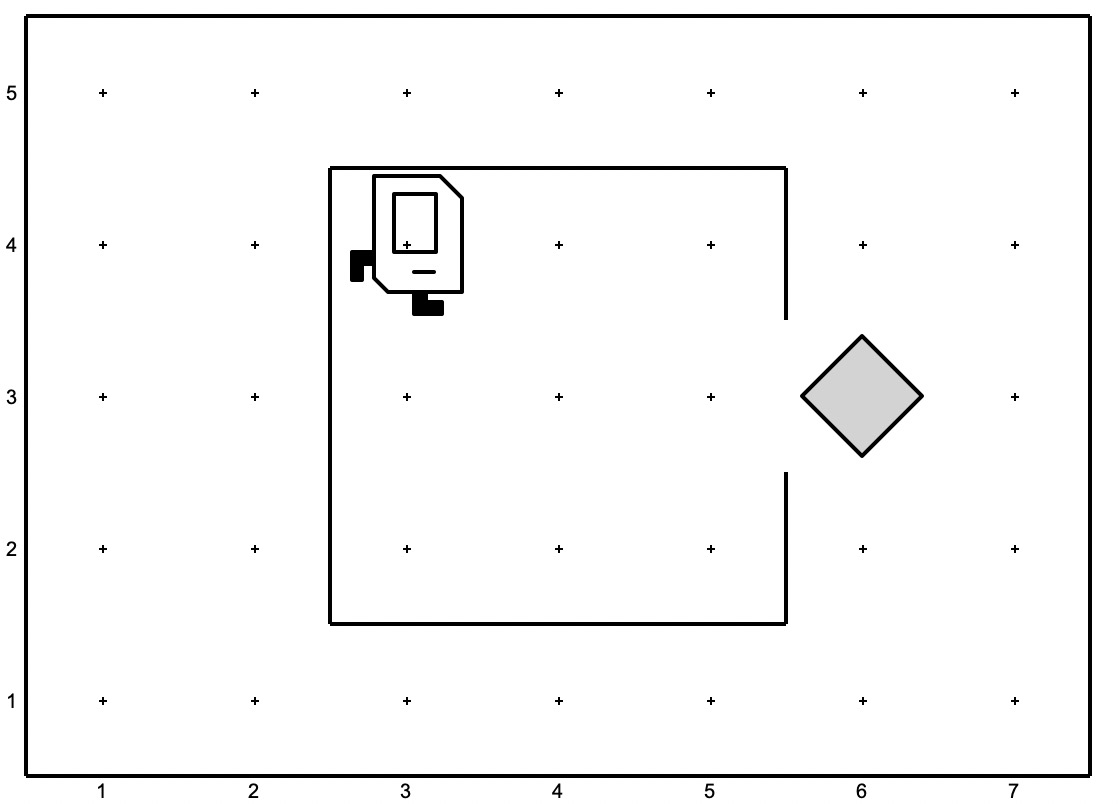
\includegraphics[width=3in, left]{ch03/PickNewspaper/init.jpg}
\end{figure}
ကားရဲလ်ကို ခြံဝင်းတံခါးဝနားရှိ သတင်းစာကို သွားပြီး ကောက်ခိုင်းမယ်။ \Fig \vref{fig:PickNewspaper} တွင် ကြည့်ပါ။ \mmcommand တွေကို ဘယ်လို အစီအစဉ်နဲ့ ပေးရမှာလဲ မစဉ်းစားသေးပဲ ဘာတွေလုပ်ခိုင်းရမှာလဲ စဉ်းစားကြည့်လျှင်
 \begin{enumerate}
   \item သတင်းစာရှိတဲ့ နေရာကိုသွား \label{itm:PickNsprGo}
   \item သတင်းစာကောက် \label{itm:PickNsprPick}
   \item နကိုမူလနေရာကို ပြန်လာ \label{itm:PickNsprBack}
 \end{enumerate}
 စသည့် အလုပ်သုံးခု အဓိကပါဝင်တယ်လို့ ပထမ အဆင့်အနေနဲ့ အကြမ်းဖျဉ်း ခွဲခြားကြည့်လို့ရမယ်။ “\ref*{itm:PickNsprGo} သတင်းစာရှိတဲ့ နေရာကိုသွား” ဖို့အတွက် လုပ်ရမယ့် အလုပ်တွေကို နောက်ထပ်တစ်ဆင့် ထပ်၍ ခွဲခြား ကြည့်ပါက
\begin{itemize}
  \item ရှေ့တည့်တည့် နံရံဆီကိုသွား
  \item ညာဘက်လှည့်
  \item ရှေ့တိုး 
  \item ဘယ်ဘက်လှည့်
  \item ‌ရှေ့တိုး 
\end{itemize}
“\ref*{itm:PickNsprPick} သတင်းစာကောက်” ဖို့အတွက် အလုပ်တွေကို ထပ်ခွဲထုတ်ကြည့်ရင်
\begin{itemize}
  \item သတင်းစာရှိ/မရှိ စစ်
  \item ရှိလျှင်ကောက် 
\end{itemize}
“\ref*{itm:PickNsprBack} နကိုမူလနေရာကို ပြန်လာ” ဖို့အတွက် ပါဝင်မယ့် အလုပ်တွေကတော့
 \begin{itemize}
  \item အနောက်ဘက်ပြန်လှည့်
  \item နံရံဆီကိုသွား 
  \item ညာဘက်လှည့်
  \item ရှေ့တိုး
  \item ညာဘက်လှည့်
\end{itemize}
စသည်ဖြင့် တွေ့နိုင်တယ်။

ဖော်ပြခဲ့သလိုမျိုး အဓိက ဖြေရှင်းရမယ့် အလုပ်\myen{(main task/problem)}ကို ပိုပြီးရိုးရှင်းတဲ့ အလုပ်တွေ\myen{(subtasks/subproblems)} အဖြစ် ခွဲထုတ်မယ်၊ ခွဲထုတ်ရရှိလာတဲ့ အလုပ်တွေကို နောက်ထပ်တစ်ဆင့် ပို၍ပို၍ ရိုးရှင်းတဲ့ အလုပ်တွေဖြစ်အောင် ထပ်ခွဲထုတ်မယ်။ ထိုကဲ့သို့ အလုပ်တစ်ခုကို ရိုးရှင်းသည်ထက် ရိုးရှင်းပြီး ဖြေရှင်းရ လွယ်ကူသည်ထက် လွယ်ကူလာတဲ့ အလုပ်တွေခွဲထုတ်တဲ့ လုပ်ငန်းစဉ်ကို \enProblemDecomposition လို့ခေါ်တယ်။

\section{\myensecttl{Top-Down Approach}}

\enProblemDecomposition နှင့် ဆက်စပ်နေတဲ့ \myen{top-down approach} ဖြင့် \mmprogram ရေးသည့် နည်းလမ်းကို ဆက်လေ့လာကြရအောင်။ ကားရဲလ်ကို တန်းကျော်ပြေး ခိုင်းမယ်။ \mmavenue အရေအတွက်က ၁၄ လမ်း ပုံသေဖြစ်မယ်။ \mmstreet အရေအတွက်က ကမ္ဘာတစ်ခုနဲ့တစ်ခု တူချင်မှ တူမယ်။ တန်းတွေရဲ့ အမြင့်နဲ့ နေရာတွေလည်း မတူဘူးလို့ ယူဆပါ။ နမူနာ ကမ္ဘာတစ်ခုကို \Fig \vref*{fig:HurdleJumping} တွင် တွေ့နိုင်တယ်။ အလားတူ အခြား ကမ္ဘာတစ်ခု အတွက်လည်း ကားရဲလ်ကို တန်းတွေ တစ်ခုချင်းစီကို ကျော်ဖြတ်ပြီး ပန်းတိုင်ဖြစ်တဲ့ (၁၄, ၁) \mmcorner ကို ရောက်အောင် သွားခိုင်းရမှာပါ။ 

\begin{figure}[h]
  \caption{\mymmfigcpt{တန်းကျော်ပြေး ပြိုင်ပွဲဝင်မည့် ကားရဲလ်၏ ကမ္ဘာ}}\label{fig:HurdleJumping}
  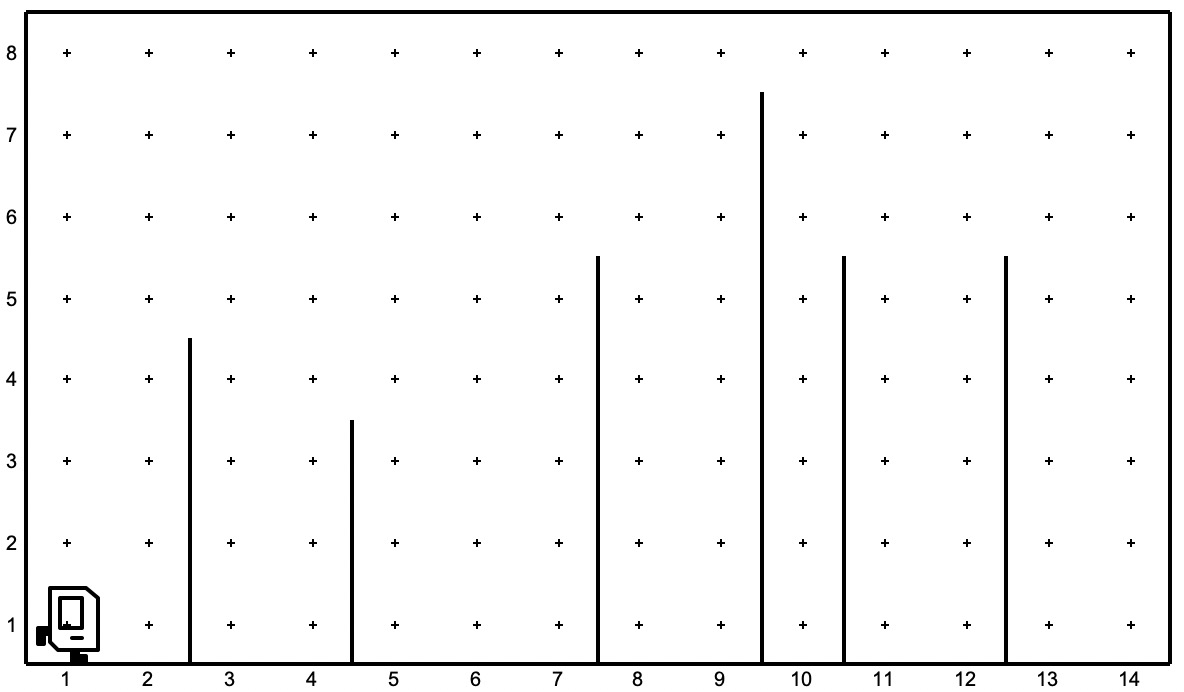
\includegraphics[width=4.5in, left]{ch03/HurdleJumping/init_w1.jpg}
\end{figure}

%\begin{lstcodesimple}[float, caption=ပထမစမ်းကြည့်ပုံ, label={lst:HurdleJumpingMain}]
%public class HurdleJumping extends stanford.karel.Karel {
%        public void run(){
%                // Karel has to move or jump over the hurdle 
%                // until (14,1). There 
%                for (int i = 0; i < 13; i++) {
%                        if (frontIsClear()) {
%                                move();
%                        } else {
%                                jumpOverAHurdle();
%                        }
%                }
%        }
%}
%\end{lstcodesimple}

\mmprogram ချမရေးသေးပဲ အဓိကအလုပ်ကို ပိုင်းခြားကြည့်လျှင် တန်းတစ်ခု ကျော်ခြင်းနှင့် ရှေ့တိုးခြင်း* အလုပ်အခွဲ နှစ်ခုကို တွေ့ရတယ်။ ရှေ့ကိုတိုးခိုင်းဖို့က \mycode{move} ကို ကားရဲလ် နားလည်ပြီးသား။ တန်းတစ်တန်း ကျော်ခိုင်းဖို့ \mycode{jumpOverAHurdle} \mmcommand သာရှိခဲ့မယ်၊ ကားရဲလ်သာ ဒီ \mmcommand ကို နားလည်ခဲ့မယ်ဆိုလျှင် 
\begin{lstcodeminimal}
for (int i = 0; i < 13; i++) {
        if (frontIsClear()) {
                move();
        } else {
                jumpOverAHurdle();
        }
}
\end{lstcodeminimal} 
ပုံစံဖြင့် ရေးနိုင်တယ်။ \mycode{jumpOverAHurdle} က တကယ်မရှိသေးတဲ့ အတွက် ဒီ \mmprogram ကို \mmrun လို့တော့ မရသေးပါဘူး။

အခု အဆင့်မှာပဲ ဒီအတိုင်းရေးထားတာ မှန်တယ်ဆိုတာ ရှေ့ဆက် မသွားခင် ဘယ်လို သေချာအောင် လုပ်လို့ရမလဲ။ စမ်းကြည့်လို့ရမလဲ။ \mycode{jumpOverAHurdle} ကလဲ အမှန်တကယ် မရှိသေးဘူး။ တစ်ခု လုပ်လို့ရတာက \mycode{jumpOverAHurdle} \mmcommand က ဘာလုပ်ပေးမှာလဲ တိတိကျကျ အရင်ဆုံး သတ်မှတ်ထားမယ်။ တနည်းအားဖြင့် ဒီ \mmcommand ကို မလုပ်ဆောင်မီနဲ့ လုပ်ဆောင်ပြီး ရှိနေရမယ့် အခြေအနေကို အတိအကျ သတ်မှတ်ထားမယ်လို့ ဆိုလိုတာပါ။ ရွေးချယ် သတ်မှတ်လို့ ရနိုင်တဲ့ အခြေအနေ နှစ်ခုစီကို \Fig \ref*{fig:jumpOverAHurdlePre}   နှင့် \ref*{fig:jumpOverAHurdlePost} တို့တွင်ကြည့်ပါ။ အဆင်ပြေနိုင်တဲ့ တစ်ခုစီကို ရွေးချယ်သတ်မှတ်ပြီး၊ သတ်မှတ်ချက်အတိုင်း \mycode{jumpOverAHurdle} လုပ်ဆောင်ပေးမယ်ဆိုလျှင် အထက်ပါ အဓိက \enForLoop ဘယ်လိုအလုပ်လုပ်မလဲ၊  \mmiteration တစ်ခေါက် ပြီးတိုင်း ဘယ်လို အခြေအနေမှာ ရှိနေမလဲ၊ နောက်ဆုံး တစ်ဆယ်သုံးကြိမ်မြောက် \mmiteration အပြီးမှာ လိုရာပန်းတိုင်ကို ကားရဲလ်ရောက်သွား မှာလား စသည်ဖြင့် တဆင့်ချင်း စစ်ကြည့်လို့ရပါတယ်။

\begin{figure}[tbh!]
  \caption{\myenlstcpt{\mycodefigcpt{jumpOverAHurdle}} \mymmfigcpt{မလုပ်ဆောင်မီ ရှိနေနိုင်သည့် အခြေအနေ နှစ်ခု}}
  \begin{subfigure}[t]{0.3\textwidth}
      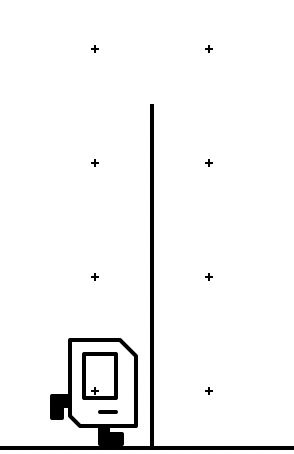
\includegraphics[width=1in, left]{ch03/HurdleJumping/JumpOverPre1.jpg}
      \caption{}
      \label{fig:JumpOverPre1}
  \end{subfigure}
  \begin{subfigure}[t]{0.3\textwidth}
      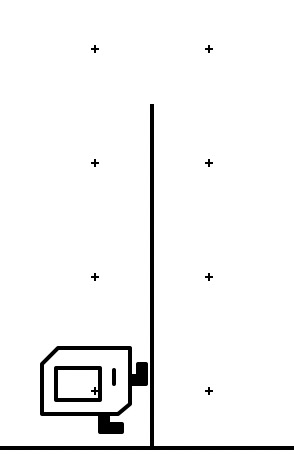
\includegraphics[width=1in, left]{ch03/HurdleJumping/JumpOverPre2.jpg}
      \caption{}
  \end{subfigure}
  \label{fig:jumpOverAHurdlePre}
\end{figure}

\begin{figure}[tbh!]
  \caption{\mycodefigcpt{jumpOverAHurdle} \mymmfigcpt{လုပ်ဆောင်ပြီး ရှိနေနိုင်သည့် အခြေအနေ နှစ်ခု}}
  \begin{subfigure}[t]{0.3\textwidth}
    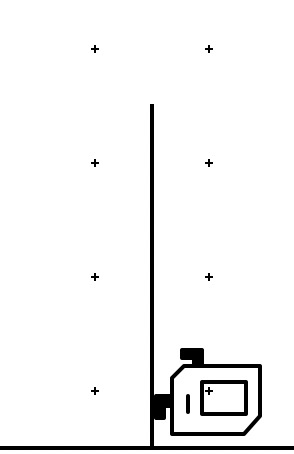
\includegraphics[width=1in, left]{ch03/HurdleJumping/JumpOverPost1.jpg}
    \caption{}
    \label{fig:JumpOverPost1}
  \end{subfigure}
  \begin{subfigure}[t]{0.3\textwidth}
      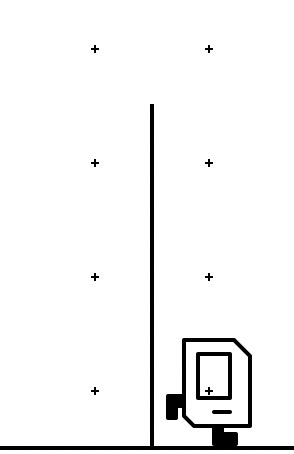
\includegraphics[width=1in, left]{ch03/HurdleJumping/JumpOverPost2.jpg}
      \caption{}
  \end{subfigure}
  \label{fig:jumpOverAHurdlePost}
\end{figure}

\Fig \ref*{fig:JumpOverPre1} နှင့် \ref*{fig:JumpOverPost1} ကို မလုပ်ဆောင်မီနှင့် လုပ်ဆောင်ပြီး အခြေအနေတွေအဖြစ် ရွေးချယ်သတ်မှတ်တယ်လို့ ယူဆပြီး \mmiteration တစ်ခါပြီးတိုင်း ရှိနေမည့် အခြေအနေကို လိုက်ကြည့်လျှင် \Fig \ref{fig:HurdleJumpingIters} မှာပြထားတဲ့ အတိုင်း တွေ့ရမယ်။ \enForLoop ပထမ တစ်ကျော့မှာ \mycode{move();}  ဒုတိယ တစ်ကျော့တွင် \mycode{jumpOverAHurdle();} လုပ်ဆောင်မည်ဖြစ်ပြီး \Fig \ref*{fig:HurdleJumping1stIter} နှင့် \ref*{fig:HurdleJumping2ndIter} တို့သည် သတ်မှတ်ထားသော \mycode{jumpOverAHurdle} မလုပ်ဆောင်မီနှင့် လုပ်ဆောင်ပြီး အခြေနေတို့ဖြင့် ကိုက်ညီကြောင်း သတိပြုပါ။ ထို့အတူ တတိယ အကျော့မှာ \mycode{move();}  စတုတ္ထ အကျော့တွင် \mycode{jumpOverAHurdle();}ကို လုပ်ဆောင်မည်ဖြစ်ပြီး \Fig \ref*{fig:HurdleJumping3rdIter} နှင့် \Fig \ref*{fig:HurdleJumping4thIter} တို့သည် သတ်မှတ်ထားသော \mycode{jumpOverAHurdle} မလုပ်ဆောင်မီနှင့် လုပ်ဆောင်ပြီး အခြေနေတို့ဖြင့် ကိုက်ညီတယ်။
\begin{figure}[!htb]
  \caption{\mymmfigcpt{\mmiteration လေးခု}}
  \begin{subfigure}[t]{0.3\textwidth}
      \adjincludegraphics[height=2in,trim={0 0 {.61\width} 0}, clip, left]{ch03/HurdleJumping/init_w1.jpg}
      \caption{}
      \label{fig:HurdleJumpingInit}
  \end{subfigure}
  \begin{subfigure}[t]{0.3\textwidth}
    \adjincludegraphics[height=2in,trim={0 0 {.61\width} 0}, clip, left]{ch03/HurdleJumping/1st_iter.jpg}
      \caption{}
      \label{fig:HurdleJumping1stIter}
  \end{subfigure}
  \begin{subfigure}[t]{0.3\textwidth}
    \adjincludegraphics[height=2in,trim={0 0 {.61\width} 0}, clip, left]{ch03/HurdleJumping/2nd_iter.jpg}
    \caption{}
    \label{fig:HurdleJumping2ndIter}
\end{subfigure}
\hspace{0.1in}
\begin{subfigure}[t]{0.3\textwidth}
  \adjincludegraphics[height=2in,trim={0 0 {.61\width} 0}, clip, left]{ch03/HurdleJumping/3rd_iter.jpg}
    \caption{}
    \label{fig:HurdleJumping3rdIter}
\end{subfigure}
\begin{subfigure}[t]{0.3\textwidth}
  \adjincludegraphics[height=2in,trim={0 0 {.61\width} 0}, clip, left]{ch03/HurdleJumping/4th_iter.jpg}
    \caption{}
    \label{fig:HurdleJumping4thIter}
\end{subfigure}
\label{fig:HurdleJumpingIters}
\end{figure}

ဒီအတိုင်းသာ \mycode{jumpOverAHurdle}  အလုပ်လုပ်မယ်ဆိုလျှင် ရှေ့မှာ တွေ့ခဲ့တဲ့ \enForLoop အရ ကားရဲလ်ဟာ တန်းတွေကျာ်ပြီး ပန်းတိုင်ရောက်မှာပါ။ ဒါပေမယ့် \mycode{jumpOverAHurdle} က အမှန်တကယ် မရှိသေးပါဘူး။ ဒီ\mmcommand\ ဘာလုပ်ပေးမလဲ ဆိုတာကိုပဲ တိတိကျကျ သတ်မှတ်ပြီး \enForLoop တစ်ကျော့ပြီးတစ်ကျော့ ရှိနေမယ့် အခြေအနေကို လိုက်ကြည့်ပြီး \mmprogram မှန်မှန်ကန်ကန် အလုပ် လုပ်/မလုပ် စစ်ကြည့်ခဲ့တာပါ။ 

ဒုတိယ အဆင့်မှာ \mycode{jumpOverAHurdle} ကို ဘယ်လိုဖြေရှင်းမလဲ ဆက်ပြီးစဉ်းစားကြမယ်။ အဓိကဖြစ်တဲ့ တန်းအားလုံးအား ကျော်ခြင်း အလုပ်ကို အလုပ်ခွဲတွေအဖြစ် ပိုင်းခြားကြည့်ခဲ့သလိုပဲ တန်းတစ်ခုအား ကျော်ခြင်း အလုပ်ခွဲကိုလည်း အပေါ်တက်ခြင်းနဲ့ အောက်ဆင်းခြင်း ဆိုပြီး ထပ်၍ ပိုင်းခြား ကြည့်လို့ရပါတယ်။ ဒီအလုပ်အခွဲ နှစ်ခုကို လုပ်ဆောင်ပေးမယ့် \mmcommand တွေကို \mycode{ascend} နဲ့ \mycode{descend} လို့ အမည်ပေးမယ်။ ဒီ \mmcommand နှစ်ခုကိုလည်း ရှိပြီးသကဲ့သို့ မှတ်ယူမယ်။ ဘယ်လို လုပ်ဆောင်မှာလဲ မစဉ်းစားသေးပဲ ဘာလုပ်ပေးမှာလဲ အရင်သတ်မှတ်ပါမယ်။
\begin{figure}[!htb]
  \caption{\myenlstcpt{\mycodefigcpt{ascend}} \mymmfigcpt{မလုပ်ဆောင်မီနှင့် လုပ်ဆောင်ပြီး}}
  \begin{subfigure}[t]{0.3\textwidth}
      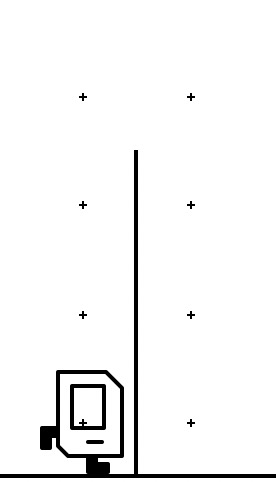
\includegraphics[width=1in, left]{ch03/HurdleJumping/ascendPre.jpg}
      \caption{}
  \end{subfigure}
  \begin{subfigure}[t]{0.3\textwidth}
      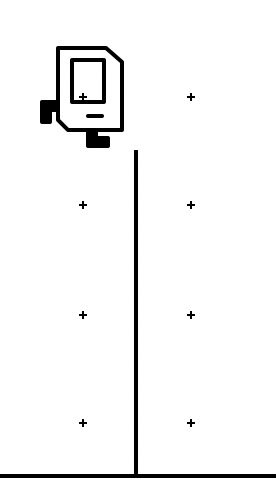
\includegraphics[width=1in, left]{ch03/HurdleJumping/ascendPost.jpg}
      \caption{}
  \end{subfigure}
  \label{fig:ascendPreAndPost}
\end{figure}
\begin{figure}[!htb]
  \caption{\myenlstcpt{\mycodefigcpt{descend}} \mymmfigcpt{မလုပ်ဆောင်မီနှင့် လုပ်ဆောင်ပြီး}}
  \begin{subfigure}[t]{0.3\textwidth}
    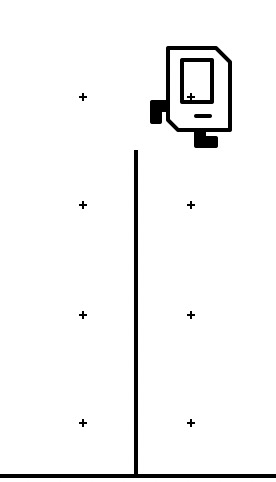
\includegraphics[width=1in, left]{ch03/HurdleJumping/descendPre}
    \caption{}
  \end{subfigure}
  \begin{subfigure}[t]{0.3\textwidth}
      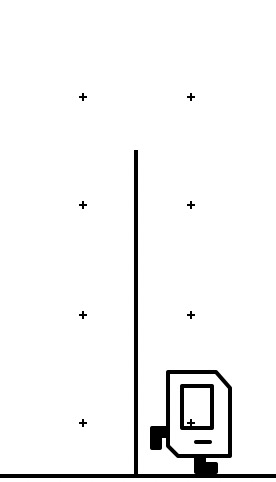
\includegraphics[width=1in, left]{ch03/HurdleJumping/descendPost}
      \caption{}
  \end{subfigure}
  \label{fig:descendPreAndPost}
\end{figure}
\Fig \ref*{fig:ascendPreAndPost}   နှင့် \ref*{fig:descendPreAndPost} တို့တွင် ပြထားသလို သတ်မှတ်မယ်။ ဒီအတိုင်းသတ်မှတ်မှ ရမယ်လို့ မဆိုလိုဘူး။ စိတ်ကြိုက် အဆင်ပြေမယ့် အနေအထားကို ရွေးချယ် သတ်မှတ်နိုင်ပါတယ်။ ပုံသေမရှိပါဘူး။ သတ်မှတ်ထားတဲ့ အတိုင်း လုပ်ဆောင်ပေးမယ်လို့ ယူဆပြီး \mycode{jumpOverAHurdle} ကို အခုလို ရေးနိုင်တယ်။ 
\begin{lstcodeminimal}
private void jumpOverAHurdle(){
        ascend(); 
        move(); //// Required!
        descend();
}
\end{lstcodeminimal}
\mycode{ascend} အပြီးမှာ \mycode{descend} မလုပ်ဆောင်မီ ရှိနေရမယ့် သတ်မှတ်ထားတဲ့ အခြေအနေနဲ့ ကိုက်ညီဖို့အတွက် အတွက်  \mycode{move();} \mmcommand လိုအပ်တာကို သတိပြုပါ။ 

အခုဆက်ပြီး ဖြေရှင်းရမှာက \mycode{ascend} နဲ့ \mycode{descend} ပါ။ ဒီအလုပ် နှစ်ခုကို ပိုပြီး ရိုးရှင်းတဲ့ အလုပ်တွေဖြစ်အောင် ထပ်ပြီး ခွဲခြမ်းကြည့်လို့ ရမလား သို့ မဟုတ် ခွဲခြမ်းကြည့်သင့် မလား  စဉ်းစားရမယ်။ ဘယ်လောက်ရိုးရှင်းတဲ့ အလုပ်ခွဲတွေ ဖြစ်လာတဲ့ အထိ ဒီအတိုင်းဆက်ပြီး ခွဲနေရမလဲ။ ဘယ်အခါမှာ အလုပ်အခွဲ အသစ်တွေ ရှာနေတာကို ရပ်ရမလဲ။ ဒါ‌တွေကလဲ စဉ်းစား ရမယ့် အချက်တွေပါ။ 

လက်ရှိအဆင့်မှာ အလုပ်အခွဲကို \mmcommand တစ်ခု အနေနဲ့ ရေးရတာ မခက်တော့ဘူး၊ အတန်အသင့် လွယ်လွယ်ကူကူ ရေးလို့ရပြီဟု ယူဆလျှင် သော်လည်းကောင်း၊ လက်ရှိ ထပ်မံ ပိုင်းခြားရန် စဉ်းစားမည့် အလုပ်အခွဲကို ဖွဲ့စည့်ထားသည့် ပို၍ရိုးရှင်းသော အလုပ်အခွဲငယ်များ၏ အမည်ကို စဉ်းစား၍ မရတော့လျှင် သော်လည်းကောင်း ရပ်လိုက်နိုင်သည်ဟု အကြမ်းဖျဉ်း ပြောနိုင်တယ်။ 

\mycode{jumpOverAHurdle} မှာတော့ တက်တာနဲ့ ဆင်းတာ အလုပ်နှစ်ခုပါတယ်ဆိုတာ မြင်သာတယ်။ အတက်နဲ့ အဆင်း အမည်ပေးရတာလဲ သိပ်စဉ်းစားနေစရာ မလိုဘူး။ \mycode{ascend} နဲ့ \mycode{descend} ကို ဖွဲ့စည်းထားတဲ့ အလုပ်ခွဲတွေက ဘာတွေဖြစ်မလဲ။ သူတို့ထက် ပိုပြီး ရိုးရှင်းတဲ့ အလုပ်က ဘယ်ဘက်လှည့်တာ၊ ညာဘက်လှည့်တာ ရှိမယ်။ ဘယ်ဘက်လှည့်ဖို့ အတွက်က \mycode{turnLeft} ရှိထားပြီးပြီ။ ညာဘက်လှည့်ဖို့ အတွက် \mycode{turnRight} အလုပ်အခွဲ သတ်မှတ်နိုင်တယ်။ တန်းတစ်ခု ထိပ်ထိရောက်အောင် သွားဖို့အတွက် \mycode{while(rightIsBlocked())} သုံးပြီး သွားလို့ရတယ်ဆိုတာ ရှေ့အခန်းမှာ တွေ့ခဲ့ပြီးပြီ။ သိပ်လဲမခက်ဘူး။ ဖော်ပြပါ အချက်တွေကြောင့် အတက်နဲ့ အဆင်း အလုပ်နှစ်ခုကို ထပ်ပြီီးမခွဲတော့ဖို့ ဆုံးဖြတ်နိုင်ပြီး အောက်ပါအတိုင်း ရေးနိုင်တယ်။
\begin{lstcodeminimal}
private void ascend() {
        turnLeft();
        while (rightIsBlocked()) {
                move();
        }
        turnRight();
}
private void descend() {
        turnRight();
        while (frontIsClear()) {
                move();
        }
        turnLeft();
}
\end{lstcodeminimal}
ဒီအခါမှာ တန်းတွေကို တစ်ခုချင်းစီ ကျော်ပြီး ကားရဲလ်ကို ပန်းဝင်အောင် သွားခိုင်းဖို့ \mmprogram တစ်ခုလုံးလည်း ရေးပြီးသွားပါပြီ။ အပြည့်အစုံကို \Lst \ref{lst:HurdleJumpingAscDscImpl} တွင် ‌လေ့လာ ကြည့်ပါ။

\begin{lstcodelong}[{\mycodelstcpt{HurdleJumping}}, label={lst:HurdleJumpingAscDscImpl}] 
public class HurdleJumping extends stanford.karel.Karel {
        public void run(){
                for (int i = 0; i < 13; i++) {
                        if (frontIsClear()) {
                                move();
                        } else {
                                jumpOverAHurdle();
                        }
                }
        }

        private void jumpOverAHurdle(){
                ascend();
                move(); // Required!
                descend();
        }

        private void ascend() {
                turnLeft();
                while (rightIsBlocked()) {
                        move();
                }
                turnRight();
        }

        private void descend() {
                turnRight();
                while (frontIsClear()) {
                        move();
                }
                turnLeft();
        }

        private void turnRight() {
                turnLeft();
                turnLeft();
                turnLeft();
        }
}
\end{lstcodelong}

%\begin{lstcodesimple}[caption=ပထမစမ်းကြည့်ပုံ, label={lst:HurdleJumpingJumpHurdleImpl}] 
%public class HurdleJumping extends stanford.karel.Karel {
%        public void run(){
%                for (int i = 0; i < 13; i++) {
%                        if (frontIsClear()) {
%                                move();
%                        } else {
%                                jumpOverAHurdle();
%                        }
%                }
%        }
%        
%        private void jumpOverAHurdle(){
%                ascend();
%                // move(); is required due to the specified pre
%                // and post condition of ascend and descend 
%                move();
%                descend();
%        }
%}
%\end{lstcodesimple}

\mycode{HurdleJumping} \mmprogram တစ်ခုလုံး ပြီးတဲ့အထိ တဆင့်ချင်းလုပ်ခဲ့တာတွေကို ပြန်အနှစ်ချုပ် ကြည့်လျှင် အောက်ပါ   အတိုင်းတွေ့ရမယ်။ 

\begin{enumerate}
  \item တန်းအားလုံးကျော်ပြီး ပန်းတိုင်ရောက်အောင် သွားဖို့အတွက် အဓိကအလုပ်မှာ ပါဝင်တဲ့ အလုပ်အခွဲတွေ ကို စဉ်းစားတယ်။ တန်းတစ်ခု ကျော်တာသည် အလုပ်အခွဲ  ဖြစ်တယ်။  ဒီအလုပ်အခွဲကို လုပ်ဆောင်ပေးမယ့် \mmcommand ကို \mycode{jumpOverAHurdle} အမည်ပေးတယ်။ \mycode{jumpOverAHurdle} မလုပ်ဆောင်မီ ရှိရမည့် အခြေအနေနဲ့ လုပ်ဆောင်ပြီး ရှိရမည့် အခြေအနေတို့ကို သတ်မှတ်တယ်။ ဒီသတ်မှတ်ချက်တွေ အတိုင်း လုပ်ဆောင်မယ်လို့ ယူဆပြီး တန်းအားလုံးကျော်ပြီး ပန်းတိုင်ရောက်အောင် သွားဖို့အတွက်ကို ဖြေရှင်းတယ်။     \label{itm:HurdleJumpingMain}
  
  \item \mycode{jumpOverAHurdle} က ဘယ်လိုဖြေရှင်းရမလဲ ဆက်ပြီးစဉ်းစားတယ်။ တန်းတစ်ခု ကျော်တဲ့ အလုပ်ကိုလဲ အလုပ်အခွဲတွေ အဖြစ်ထပ်ပြီး ခွဲတယ်။ အပေါ်တက်နဲ့ အောက်ဆင်း နှစ်ခု ပါဝင်တာတွေ့ရတယ်။ ဒီနှစ်ခုကို လုပ်ဆောင်ပေးမယ့် \mmcommand တွေကို \mycode{ascend} နဲ့ \mycode{descend} အမည်ပေးတယ်။ \mycode{ascend} နဲ့ \mycode{descend} မလုပ်ဆောင်မီ ရှိရမည့် အခြေအနေနဲ့ လုပ်ဆောင်ပြီး ရှိရမည့် အခြေအနေတို့ကို သတ်မှတ်တယ်။ သတ်မှတ်ချက်အတိုင်း လုပ်ဆောင်မယ်လို့ ယူဆပြီး \mycode{jumpOverAHurdle} ဖြေရှင်းတယ်။     \label{itm:HurdleJumpingSub}

  \item အပေါ်တက်တဲ့ အလုပ်နဲ့ အောက်ဆင်းတဲ့ အလုပ်ကို ထပ်ပြီးခွဲကြည့်ဖို့ စဉ်းစားတယ်။ သို့ပေမယ့် အဓိပ္ပါယ်ရှိတဲ့ အလုပ်အခွဲကို နာမည်ပေးဖို့ စဉ်းစားလို့မရတော့ဘူး။ ဒါ့အပြင် ဒီအလုပ်နှစ်ခုကို \mmprogram ရေးဖို့ အတွက် အတန်အသင့် လွယ်ကူမယ်လို့လဲ ယူဆတယ်။ ဒါကြောင့် ဒီနှစ်ခုကို ဆက်မခွဲတော့ပဲ\mycode{ascend} နဲ့ \mycode{descend} တွေကို သတ်မှတ်တယ်။ 
  \label{itm:HurdleJumpingJumpSubsub}
\end{enumerate}
%\bigskip

ဖော်ပြခဲ့သလို အဓိက အလုပ်ကို ဖြေရှင်းဖို့အတွက် အလုပ်အခွဲတွေ အဖြစ်ပိုင်းခြားပြီး ရရှိလာတဲ့ အလုပ်အခွဲတွေကို လုပ်ဆောင်ပေးမယ့် \mmcommand တွေ ရှိထားပြီး ဖြစ်သကဲ့သို့ မှတ်ယူပြီး (ဒီ \mmcommand တွေဘာ လုပ်ပေးမှာလဲ၊ မလုပ်ဆောင်မီနှင့် လုပ်ဆောင်ပြီး အခြေအနေ တွေကို သတ်မှတ်ပြီး) အဓိက အလုပ်ကို ဖြေရှင်းတဲ့ နည်းလမ်းကို \mmTopDown နည်းလမ်းလို့ ခေါ်တယ်။  \enStepWiseRefinement ဟုလည်း ခေါ်တယ်။ 

ဖော်ပြခဲ့သလိုမျိုး လုပ်ငန်းစဉ်အတိုင်း နောက်ထပ် ပုစ္ဆာတစ်ခုကို ဖြေရှင်းကြည့်ရအောင်။ \Fig \ref{fig:SweepTheStreetsW1} နမူနာ ကမ္ဘာကို ပြထားတယ်။ 
\begin{figure}[!htb]
  \caption{ကားရဲလ်နှင့်  ကားရဲလ်၏ကမ္ဘာ}\label{fig:SweepTheStreetsW1}
  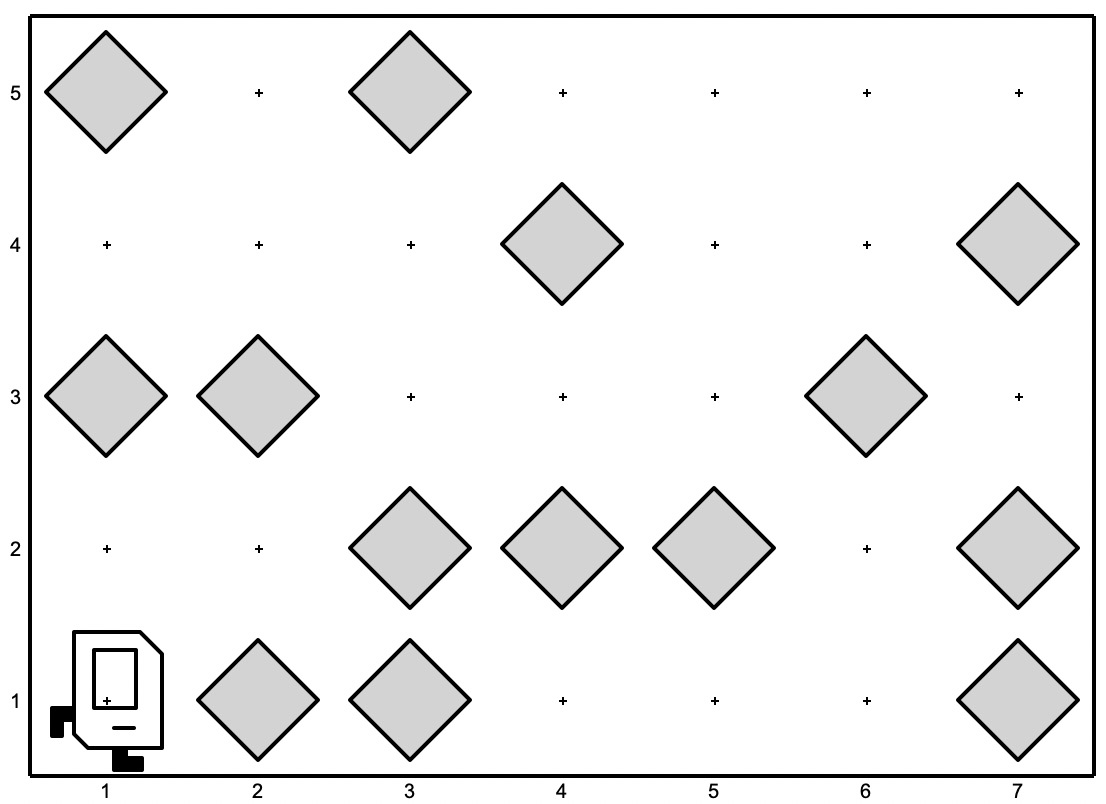
\includegraphics[width=4in, left]{ch03/SweepTheStreets/init_w1.jpg}
\end{figure}
လုပ်ရမယ့် အလုပ်က \mmbeeper တွေ ကုန်အောင် ရှင်းပေးရမှာပါ။ အလားတူ မည်သည့် $m \times n$ ကမ္ဘာတွင်မဆို အမှိုက်တွေ ကုန်အောင် ရှင်းပေးရမှာပါ။

အခန်းတစ်ခန်းလုံး ရှင်းဖို့အလုပ်မှာ တစ်လမ်းရှင်းတာ၊ မြောက်ဘက် လှည့်တာ၊ နောက်လမ်းတစ်ခု ဆက်ရှင်းဖို့အတွက် အဆင်သင့်ပြင်တာ စတဲ့ အလုပ်အခွဲ သုံးခု ပါဝင်တယ်။ ဒီအလုပ် သုံးခုကို
\begin{enumerate}
  \item \mycode{sweepOneSt}
  \item \mycode{turnNorth}
  \item \mycode{getReadyForNextSt}
\end{enumerate}
\mmcommand တွေအနေနဲ့ အသီးသီး ယူဆမယ်။ ဒီသုံးခုက ဘာလုပ်ပေးမှာလဲ အရင်ဆုံး သတ်မှတ်မယ်။ 
\begin{enumerate}
\item \mycode{sweepOneSt}
\begin{itemize}
\item လမ်းတစ်လမ်း၏ အစ သို့ အဆုံးတွင် အခြားဘက်စွန်းသို့ မျက်နှာမူပြီး ရှိနေမယ်။
\item လမ်း၏ အခြားဘက်အဆုံးသို့ ရောက်ရှိပြီး ရှေ့တွင် နံရံပိတ်နေမယ်။ \mmbeeper အားလုံး ရှင်းပြီး ဖြစ်မယ်။ \Fig \ref{fig:sweepOneStPreAndPostConds} တွင်ကြည့်ပါ။
\end{itemize}
\item \mycode{turnNorth}  
  \begin{itemize}
    \item \mmcorner တစ်ခုတွင် ရှိနေမည်။
    \item မည်သည့် အရပ်သို့ မျက်နှာမူနေသည်ဖြစ်စေ မြောက်ဘက်သို့ လှည့်ပြီးဖြစ်နေရမည်။
  \end{itemize} 
  \item \mycode{getReadyForNextSt}
  \begin{itemize}
    \item လမ်းတစ်လမ်း၏ အစ သို့ အဆုံးတွင် မြောက်ဘက်သို့ မျက်နှာမူပြီးရှိနေမည်။
    \item အပေါ်တစ်လမ်းကူးပြီး လမ်း၏ အခြားဘက်ဆုံးသို့ မျက်နှာမူပြီးရှိနေမည်။ \Fig \ref{fig:getReadyForNextPostAndPost} တွင်ကြည့်ပါ။
  \end{itemize}   
\end{enumerate}
\mmcommand သုံးခုက ဒီသတ်မှတ်ချက်တွေအတိုင်း အလုပ်လုပ်မယ်ဆိုရင် လမ်းအားလုံးရှင်းဖို့ အတွက် အခုလို ရေးလို့ရမယ်။ 
\begin{lstcodeminimal}
sweepOneSt();
while(frontIsClear()) {
        getReadyForNextSt();
        sweepOneSt();
}
\end{lstcodeminimal}

%\begin{lstcodesimple}[float=tbh!, caption=ပထမစမ်းကြည့်ပုံ, label={lst:SweepTheStreetsMain}] 
%public class SweepTheStreets extends stanford.karel.Karel {
%        public void run() {
%                cleanOneSt();
%                while(frontIsClear()) {
%                        getReadyForNextSt();
%                        cleanOneSt();
%                }
%        }
%}
%\end{lstcodesimple}

\begin{figure}[tbh!]
  \caption{\mymmfigcpt{\mmiteration လေးခု}}
  \begin{subfigure}[t]{0.48\textwidth}
      \adjincludegraphics[width=2.5in,trim={0 0 0 {.55\height}}, clip, left]{ch03/SweepTheStreets/init_w1.jpg}
      \caption{}
      \label{fig:sweepOneStPreOdd}
  \end{subfigure}
  \hspace{0.1in}
  \begin{subfigure}[t]{0.48\textwidth}
    \adjincludegraphics[width=2.5in,trim={0 0 0 {.55\height}}, clip, left]{ch03/SweepTheStreets/sweepOneStPostOdd.jpg}
      \caption{}
      \label{fig:sweepOneStPostOdd}
  \end{subfigure}

  \vspace{0.1in}
  \begin{subfigure}[t]{0.48\textwidth}
    \adjincludegraphics[width=2.5in,trim={0 0 0 {.55\height}}, clip, left]{ch03/SweepTheStreets/sweepOneStPreEven.jpg}
    \caption{}
    \label{fig:sweepOneStPreEven}
  \end{subfigure}
  \hspace{0.1in}
  \begin{subfigure}[t]{0.48\textwidth}
    \adjincludegraphics[width=2.5in,trim={0 0 0 {.55\height}}, clip, left]{ch03/SweepTheStreets/sweepOneStPostEven.jpg}
      \caption{}
      \label{fig:sweepOneStPostEven}
  \end{subfigure}
  \label{fig:sweepOneStPreAndPostConds}
\end{figure}

\begin{figure}[tbh!]
  \caption{\mymmfigcpt{\mmiteration လေးခု}}
  \begin{subfigure}[t]{0.48\textwidth}
      \adjincludegraphics[width=2.5in,trim={0 0 0 {.4\height}}, clip, left]{ch03/SweepTheStreets/getReadyForNextPreOdd.jpg}
      \caption{}
      \label{fig:getReadyForNextPreOdd}
  \end{subfigure}
  \hspace{0.1in}
  \begin{subfigure}[t]{0.48\textwidth}
    \adjincludegraphics[width=2.5in,trim={0 0 0 {.4\height}}, clip, left]{ch03/SweepTheStreets/getReadyForNextPostOdd.jpg}
      \caption{}
      \label{fig:getReadyForNextPostOdd}
  \end{subfigure}

  \vspace*{0.1in}
  \begin{subfigure}[t]{0.48\textwidth}
    \adjincludegraphics[width=2.5in,trim={0 0 0 {.4\height}}, clip, left]{ch03/SweepTheStreets/getReadyForNextPreEven.jpg}
    \caption{}
    \label{fig:getReadyForNextPreEven}
  \end{subfigure}
  \hspace{0.1in}
  \begin{subfigure}[t]{0.48\textwidth}
    \adjincludegraphics[width=2.5in,trim={0 0 0 {.4\height}}, clip, left]{ch03/SweepTheStreets/getReadyForNextPostEven.jpg}
      \caption{}
      \label{fig:getReadyForNextPostEven}
  \end{subfigure}
  \label{fig:getReadyForNextPostAndPost}
\end{figure}

\noindent ဒုတိယ  အဆင့်မှာ 
\begin{enumerate}
  \item \mycode{sweepOneSt} \label{itm:sweepOneSt}
  \item \mycode{turnNorth} \label{itm:turnNorth}
  \item \mycode{getReadyForNextSt} \label{itm:getReadyForNextSt}
\end{enumerate}
တို့ကို ဆက်ပြီး ဖြေရှင်းရမယ်။ \mycode{sweepOneSt} ကိုခွဲကြည့်မယ် ဆိုလျှင် \mmcorner တစ်ခုကို တံမြက်စည်း စင်အောင်လှည်းတာ ပါဝင်မယ်။ ဒီအလုပ်ကို \mycode{sweepOneCnr} ဟု အမည်ပေးရအောင်။ \mycode{turnNorth} ကိုတော့ အတန်အသင့် လွယ်ကူတဲ့အတွက် ထပ်မခွဲတော့ဘူး။ \mycode{getReadyForNextSt} ကိုတော့ အနောက်ဘက် လှည့်ခိုင်းခြင်း၊ အရှေ့ဘက် လှည့်ခိုင်းခြင်း ပါဝင်နေတယ်လို့ ယူဆနိုင်ပြီး \mycode{turnEast} နဲ့ \mycode{turnWest} လို့ အမည်ပေးမယ်။ *။ မလုပ်ဆောင်မီ နှင့် လုပ်ဆောင်ပြီး အခြေအနေတွေက ပေးထားတဲ့ အမည်ကနေတဆင့် သိသာနေပြီး ဖြစ်တဲ့အတွက် မဖော်ပြတော့ပဲ \Lst \ref{lst:SweepTheStreets} \mmprogram တစ်ခုလုံး အပြည့်အစုံ တွေ့နိုင်ပါတယ်။ 

\begin{lstcodelong}[{\mycodelstcpt{SweepTheStreets}}, label={lst:SweepTheStreets}] 
public class SweepTheStreets extends stanford.karel.Karel {
        public void run() {
                sweepOneSt();
                while(frontIsClear()) {
                        getReadyForNextSt();
                        sweepOneSt();
                }
        }

        private void sweepOneSt() {
                sweepOneCnr();
                while (frontIsClear()) {
                        move();
                        sweepOneCnr();
                }
                turnNorth();
        }

        private void sweepOneCnr() {
                while (beepersPresent()) {
                        pickBeeper();
                }
        }

        private void turnNorth() {
                while (notFacingNorth()) {
                        turnLeft();
                }
        }

        private void getReadyForNextSt() {
                move();
                if (rightIsBlocked()) {
                        turnWest();
                }
                if (leftIsBlocked()) {
                        turnEast();
                }
        }

        private void turnWest() {
                while(notFacingWest()) {
                        turnLeft();
                }
        }

        private void turnEast() {
                while(notFacingEast()) {
                        turnLeft();
                }
        }
}
\end{lstcodelong}

\mmcorner တစ်ခုမှာ စုပုံထားတဲ့ \mmbeeper တွေကို နှစ်ဆဖြစ်သွားအောင် ကားရဲလ်ကို လုပ်ခိုင်းချင်တယ်။ ကားရဲလ်က သင်္ချာတော့ အားနည်းပါတယ်။ ရေတွက်တာ \myen{(counting)} နဲ့ ပေါင်းနှုတ်မြှောက်စား စတာတွေ နားမလည်ဘူး။ မှတ်ထားနိုင်တဲ့ မှတ်ညာဏ်လည်း သူ့မှာမရှိဘူး။ အခြားနည်းလမ်း ရှာပြီးခိုင်းရမယ်။ ပုံထားတဲ့ နေရာက \mmbeeper တစ်ခုချင်းစီကို ကောက်ပြီး ရှေ့ \mmcorner မှာ နှစ်ခုပြန်ချ*။ ဒါကို နကိုနေရာက  \mmbeeper တွေကုန်တဲ့ အထိ လုပ်လျှင် နကို ပုံထားတဲ့ နေရာရှေ့တစ် \mmcorner မှာ နှစ်ဆပိုများတဲ့ \mmbeeper တွေ ပုံးထားပြီးဖြစ်နေမယ်။ အဲဒီ \mmbeeper တွေကို နကိုနေရာကို ပြန်ရွှေ့လိုက်ရင် ခိုင်းချင်တဲ့ အလုပ်ပြီးပါပြီ။ ပထမအဆင့် အလုပ်တွေကို ခွဲကြည့်လျှင်

\begin{enumerate}
  \item \mycode{goToBeeperPile}
  \item \mycode{doubleTheBeeperPileAtNxtCnr}
  \item \mycode{moveTheBeeperPileAtNxtCnr}
\end{enumerate}
\mmcommand တွေအနေနဲ့ အသီးသီး ယူဆမယ်။ ဒီသုံးခုက ဘာလုပ်ပေးမှာလဲ အရင်ဆုံး သတ်မှတ်မယ်။ 
\begin{enumerate}
  \item \mycode{goToBeeperPile}
  \begin{itemize}
    \item (၁, ၁) \mmcorner တွင် အရှေ့ဘက် မျက်နှာမူပြီး ရှိနေမယ်။
    \item \mmbeeper များပုံထားသည့် \mmcorner တွင် အရှေ့ဘက်သို့ မျက်နှာမူပြီး ရှိနေမယ်။။ \Fig \ref{fig:goToBeeperPilePreAndPost} တွင်ကြည့်ပါ။
  \end{itemize}
  \item \mycode{doubleTheBeeperPileAtNxtCnr}  
    \begin{itemize}
      \item \mmbeeper များ ပုံထားသည့် \mmcorner  တွင်ရှိနေသည်။
      \item ရှေ့တစ် \mmcorner တွင် \mmbeeper အရေအတွက် နှစ်ဆရှိနေပြီး အရှေ့ဘက်သို့ မျက်နှာမူ၍ နေမည်။ \Fig \ref{fig:doubleTheBeeperPileAtNxtCnrPreAndPost} တွင်ကြည့်ပါ။
    \end{itemize} 
  \item \mycode{moveTheBeeperPileAtNxtCnr}
    \begin{itemize}
      \item \mmbeeper များ ပုံထားသည့် \mmcorner  တွင် နောက်ဘက်သို့ မျက်နှာမူ၍ ရှိနေသည်။
      \item ရှေ့တစ် \mmcorner တွင် \mmbeeper များရောက်သွားပြီး အနောက်ဘက်သို့ မျက်နှာမူ၍ ရှိနေမည်။  \Fig \ref{fig:moveTheBeeperPileAtNxtCnrPreAndPost} တွင်ကြည့်ပါ။
    \end{itemize}   
\end{enumerate}

\begin{figure}[tbh!]
  \caption{\mymmfigcpt{\mycodefigcpt{goToBeeperPile} \mymmfigcpt{မလုပ်ဆောင်မီ က) နှင့် လုပ်ဆောင်ပြီး ခ)}}}
  \begin{subfigure}[t]{0.48\textwidth}
      \adjincludegraphics[width=2.5in,trim={0 0 0 {.4\height}}, clip, left]{ch03/DoubleBeeperPile/goToBeeperPilePre.jpg}
      \caption{}
      \label{fig:goToBeeperPilePre}
  \end{subfigure}
  \hspace{0.1in}
  \begin{subfigure}[t]{0.48\textwidth}
    \adjincludegraphics[width=2.5in,trim={0 0 0 {.4\height}}, clip, left]{ch03/DoubleBeeperPile/goToBeeperPilePost.jpg}
      \caption{}
      \label{fig:goToBeeperPilePost}
  \end{subfigure}
  \label{fig:goToBeeperPilePreAndPost}
\end{figure}
\begin{figure}[tbh!]
  \caption{\mymmfigcpt{\mycodefigcpt{doubleTheBeeperPileAtNxtCnr} \mymmfigcpt{မလုပ်ဆောင်မီ က) နှင့် လုပ်ဆောင်ပြီး ခ)}}}
  \begin{subfigure}[t]{0.48\textwidth}
      \adjincludegraphics[width=2.5in,trim={0 0 0 {.4\height}}, clip, left]{ch03/DoubleBeeperPile/doubleTheBeeperPileAtNxtCnrPre.jpg}
      \caption{}
      \label{fig:doubleTheBeeperPileAtNxtCnrPre}
  \end{subfigure}
  \hspace{0.1in}
  \begin{subfigure}[t]{0.48\textwidth}
    \adjincludegraphics[width=2.5in,trim={0 0 0 {.4\height}}, clip, left]{ch03/DoubleBeeperPile/doubleTheBeeperPileAtNxtCnrPost.jpg}
      \caption{}
      \label{fig:doubleTheBeeperPileAtNxtCnrPost}
  \end{subfigure}
  \label{fig:doubleTheBeeperPileAtNxtCnrPreAndPost}
\end{figure}
\begin{figure}[tbh!]
  \caption{\mymmfigcpt{\mycodefigcpt{moveTheBeeperPileAtNxtCnr} \mymmfigcpt{မလုပ်ဆောင်မီ က) နှင့် လုပ်ဆောင်ပြီး ခ)}}}
  \begin{subfigure}[t]{0.48\textwidth}
      \adjincludegraphics[width=2.5in,trim={0 0 0 {.4\height}}, clip, left]{ch03/DoubleBeeperPile/moveTheBeeperPileAtNxtCnrPre.jpg}
      \caption{}
      \label{fig:moveTheBeeperPileAtNxtCnrPre}
  \end{subfigure}
  \hspace{0.1in}
  \begin{subfigure}[t]{0.48\textwidth}
    \adjincludegraphics[width=2.5in,trim={0 0 0 {.4\height}}, clip, left]{ch03/DoubleBeeperPile/moveTheBeeperPileAtNxtCnrPost.jpg}
      \caption{}
      \label{fig:moveTheBeeperPileAtNxtCnrPost}
  \end{subfigure}
  \label{fig:moveTheBeeperPileAtNxtCnrPreAndPost}
\end{figure}

\begin{figure}[tbh!]
  \caption{\mymmfigcpt{\mycodefigcpt{moveOneBeeperAtNxtCnr} \mymmfigcpt{မလုပ်ဆောင်မီ က) နှင့် လုပ်ဆောင်ပြီး ခ)}}}
  \begin{subfigure}[t]{0.48\textwidth}
      \adjincludegraphics[width=2.5in,trim={0 0 0 {.4\height}}, clip, left]{ch03/DoubleBeeperPile/moveOneBeeperAtNxtCnrPre.jpg}
      \caption{}
      \label{fig:moveOneBeeperAtNxtCnrPostPre}
  \end{subfigure}
  \hspace{0.1in}
  \begin{subfigure}[t]{0.48\textwidth}
    \adjincludegraphics[width=2.5in,trim={0 0 0 {.4\height}}, clip, left]{ch03/DoubleBeeperPile/ moveOneBeeperAtNxtCnrPost.jpg}
      \caption{}
      \label{fig:moveOneBeeperAtNxtCnrPost}
  \end{subfigure}
  \label{fig:moveOneAtNxtCnrPreAndPost}
\end{figure}

\begin{figure}[tbh!]
  \caption{\mymmfigcpt{\mycodefigcpt{doubleOneBeeperAtNxtCnr} \mymmfigcpt{မလုပ်ဆောင်မီ က) နှင့် လုပ်ဆောင်ပြီး ခ)}}}
  \begin{subfigure}[t]{0.48\textwidth}
      \adjincludegraphics[width=2.5in,trim={0 0 0 {.4\height}}, clip, left]{ch03/DoubleBeeperPile/doubleOneBeeperAtNxtCnrPre.jpg}
      \caption{}
      \label{fig:doubleOneBeeperAtNxtCnrPre}
  \end{subfigure}
  \hspace{0.1in}
  \begin{subfigure}[t]{0.48\textwidth}
    \adjincludegraphics[width=2.5in,trim={0 0 0 {.4\height}}, clip, left]{ch03/DoubleBeeperPile/doubleOneBeeperAtNxtCnrPost.jpg}
      \caption{}
      \label{fig:doubleOneBeeperAtNxtCnrPost}
  \end{subfigure}
  \label{fig:doubleOneBeeperAtNxtCnrPreAndPost}
\end{figure}

\begin{figure}[tbh!]
  \caption{\mymmfigcpt{\mmiteration လေးခု}}
  \begin{subfigure}[t]{0.48\textwidth}
      \adjincludegraphics[width=2.5in,trim={0 0 0 {.4\height}}, clip, left]{ch03/DoubleBeeperPile/getReadyForNxtPre1.jpg}
      \caption{}
      \label{fig:getReadyForNxtPre1}
  \end{subfigure}
  \hspace{0.1in}
  \begin{subfigure}[t]{0.48\textwidth}
    \adjincludegraphics[width=2.5in,trim={0 0 0 {.4\height}}, clip, left]{ch03/DoubleBeeperPile/getReadyForNxtPost1.jpg}
      \caption{}
      \label{fig:getReadyForNxtPost1}
  \end{subfigure}
  \begin{subfigure}[t]{0.48\textwidth}
    \adjincludegraphics[width=2.5in,trim={0 0 0 {.4\height}}, clip, left]{ch03/DoubleBeeperPile/getReadyForNxtPre2.jpg}
    \caption{}
    \label{fig:getReadyForNxtPre2}
  \end{subfigure}
  \hspace{0.1in}
  \begin{subfigure}[t]{0.48\textwidth}
    \adjincludegraphics[width=2.5in,trim={0 0 0 {.4\height}}, clip, left]{ch03/DoubleBeeperPile/getReadyForNxtPost2.jpg}
      \caption{}
      \label{fig:getReadyForNxtPost2}
  \end{subfigure}
  \label{fig:getReadyForNxtPreAndPost}
\end{figure}

\begin{lstcodelong}[caption=ပထမစမ်းကြည့်ပုံ, label={lst:DoubleBeeperPileFull}] 
public class DoubleBeeperPile extends stanford.karel.Karel {
        public void run() {
                goToBeeperPile();
                doubleTheBeeperPileAtNxtCnr();
                turnAround();
                moveTheBeeperPileAtNxtCnr();
                turnAround();
        }

        private void goToBeeperPile() {
                while(noBeepersPresent()) {
                        move();
                }
        }

        private void doubleTheBeeperPileAtNxtCnr() {
                while(beepersPresent()) {
                        doubleOneBeeperAtNxtCnr();
                        getReadyForNxt();
                }
                move();
        }

        private void moveTheBeeperPileAtNxtCnr() {
                while(beepersPresent()) {
                        moveOneBeeperAtNxtCnr();
                        getReadyForNxt();
                }
                move();
        }
        private void moveOneBeeperAtNxtCnr() {
                if(beepersPresent()) {
                        pickBeeper();
                }
                move();
                putBeeper();
        }
        
        private void doubleOneBeeperAtNxtCnr() {
                if(beepersPresent()) {
                        pickBeeper();
                }
                move();
                putBeeper();
                putBeeper();
        }

        private void getReadyForNxt() {
                turnAround();
                move();
                turnAround();
        }

        private void turnAround() {
                turnLeft();
                turnLeft();
        }
}
\end{lstcodelong}
\end{sloppypar}
